\documentclass[]{article}
\usepackage{lmodern}
\usepackage{amssymb,amsmath}
\usepackage{ifxetex,ifluatex}
\usepackage{fixltx2e} % provides \textsubscript
\ifnum 0\ifxetex 1\fi\ifluatex 1\fi=0 % if pdftex
  \usepackage[T1]{fontenc}
  \usepackage[utf8]{inputenc}
\else % if luatex or xelatex
  \ifxetex
    \usepackage{mathspec}
  \else
    \usepackage{fontspec}
  \fi
  \defaultfontfeatures{Ligatures=TeX,Scale=MatchLowercase}
\fi
% use upquote if available, for straight quotes in verbatim environments
\IfFileExists{upquote.sty}{\usepackage{upquote}}{}
% use microtype if available
\IfFileExists{microtype.sty}{%
\usepackage{microtype}
\UseMicrotypeSet[protrusion]{basicmath} % disable protrusion for tt fonts
}{}
\usepackage[margin=1in]{geometry}
\usepackage{hyperref}
\hypersetup{unicode=true,
            pdfborder={0 0 0},
            breaklinks=true}
\urlstyle{same}  % don't use monospace font for urls
\usepackage{color}
\usepackage{fancyvrb}
\newcommand{\VerbBar}{|}
\newcommand{\VERB}{\Verb[commandchars=\\\{\}]}
\DefineVerbatimEnvironment{Highlighting}{Verbatim}{commandchars=\\\{\}}
% Add ',fontsize=\small' for more characters per line
\usepackage{framed}
\definecolor{shadecolor}{RGB}{248,248,248}
\newenvironment{Shaded}{\begin{snugshade}}{\end{snugshade}}
\newcommand{\KeywordTok}[1]{\textcolor[rgb]{0.13,0.29,0.53}{\textbf{#1}}}
\newcommand{\DataTypeTok}[1]{\textcolor[rgb]{0.13,0.29,0.53}{#1}}
\newcommand{\DecValTok}[1]{\textcolor[rgb]{0.00,0.00,0.81}{#1}}
\newcommand{\BaseNTok}[1]{\textcolor[rgb]{0.00,0.00,0.81}{#1}}
\newcommand{\FloatTok}[1]{\textcolor[rgb]{0.00,0.00,0.81}{#1}}
\newcommand{\ConstantTok}[1]{\textcolor[rgb]{0.00,0.00,0.00}{#1}}
\newcommand{\CharTok}[1]{\textcolor[rgb]{0.31,0.60,0.02}{#1}}
\newcommand{\SpecialCharTok}[1]{\textcolor[rgb]{0.00,0.00,0.00}{#1}}
\newcommand{\StringTok}[1]{\textcolor[rgb]{0.31,0.60,0.02}{#1}}
\newcommand{\VerbatimStringTok}[1]{\textcolor[rgb]{0.31,0.60,0.02}{#1}}
\newcommand{\SpecialStringTok}[1]{\textcolor[rgb]{0.31,0.60,0.02}{#1}}
\newcommand{\ImportTok}[1]{#1}
\newcommand{\CommentTok}[1]{\textcolor[rgb]{0.56,0.35,0.01}{\textit{#1}}}
\newcommand{\DocumentationTok}[1]{\textcolor[rgb]{0.56,0.35,0.01}{\textbf{\textit{#1}}}}
\newcommand{\AnnotationTok}[1]{\textcolor[rgb]{0.56,0.35,0.01}{\textbf{\textit{#1}}}}
\newcommand{\CommentVarTok}[1]{\textcolor[rgb]{0.56,0.35,0.01}{\textbf{\textit{#1}}}}
\newcommand{\OtherTok}[1]{\textcolor[rgb]{0.56,0.35,0.01}{#1}}
\newcommand{\FunctionTok}[1]{\textcolor[rgb]{0.00,0.00,0.00}{#1}}
\newcommand{\VariableTok}[1]{\textcolor[rgb]{0.00,0.00,0.00}{#1}}
\newcommand{\ControlFlowTok}[1]{\textcolor[rgb]{0.13,0.29,0.53}{\textbf{#1}}}
\newcommand{\OperatorTok}[1]{\textcolor[rgb]{0.81,0.36,0.00}{\textbf{#1}}}
\newcommand{\BuiltInTok}[1]{#1}
\newcommand{\ExtensionTok}[1]{#1}
\newcommand{\PreprocessorTok}[1]{\textcolor[rgb]{0.56,0.35,0.01}{\textit{#1}}}
\newcommand{\AttributeTok}[1]{\textcolor[rgb]{0.77,0.63,0.00}{#1}}
\newcommand{\RegionMarkerTok}[1]{#1}
\newcommand{\InformationTok}[1]{\textcolor[rgb]{0.56,0.35,0.01}{\textbf{\textit{#1}}}}
\newcommand{\WarningTok}[1]{\textcolor[rgb]{0.56,0.35,0.01}{\textbf{\textit{#1}}}}
\newcommand{\AlertTok}[1]{\textcolor[rgb]{0.94,0.16,0.16}{#1}}
\newcommand{\ErrorTok}[1]{\textcolor[rgb]{0.64,0.00,0.00}{\textbf{#1}}}
\newcommand{\NormalTok}[1]{#1}
\usepackage{longtable,booktabs}
\usepackage{graphicx,grffile}
\makeatletter
\def\maxwidth{\ifdim\Gin@nat@width>\linewidth\linewidth\else\Gin@nat@width\fi}
\def\maxheight{\ifdim\Gin@nat@height>\textheight\textheight\else\Gin@nat@height\fi}
\makeatother
% Scale images if necessary, so that they will not overflow the page
% margins by default, and it is still possible to overwrite the defaults
% using explicit options in \includegraphics[width, height, ...]{}
\setkeys{Gin}{width=\maxwidth,height=\maxheight,keepaspectratio}
\IfFileExists{parskip.sty}{%
\usepackage{parskip}
}{% else
\setlength{\parindent}{0pt}
\setlength{\parskip}{6pt plus 2pt minus 1pt}
}
\setlength{\emergencystretch}{3em}  % prevent overfull lines
\providecommand{\tightlist}{%
  \setlength{\itemsep}{0pt}\setlength{\parskip}{0pt}}
\setcounter{secnumdepth}{0}
% Redefines (sub)paragraphs to behave more like sections
\ifx\paragraph\undefined\else
\let\oldparagraph\paragraph
\renewcommand{\paragraph}[1]{\oldparagraph{#1}\mbox{}}
\fi
\ifx\subparagraph\undefined\else
\let\oldsubparagraph\subparagraph
\renewcommand{\subparagraph}[1]{\oldsubparagraph{#1}\mbox{}}
\fi

%%% Use protect on footnotes to avoid problems with footnotes in titles
\let\rmarkdownfootnote\footnote%
\def\footnote{\protect\rmarkdownfootnote}

%%% Change title format to be more compact
\usepackage{titling}

% Create subtitle command for use in maketitle
\providecommand{\subtitle}[1]{
  \posttitle{
    \begin{center}\large#1\end{center}
    }
}

\setlength{\droptitle}{-2em}

  \title{}
    \pretitle{\vspace{\droptitle}}
  \posttitle{}
    \author{}
    \preauthor{}\postauthor{}
    \date{}
    \predate{}\postdate{}
  

\begin{document}

ENGG 6150 Term Project Component Design 4\\
Student: Jian Bin(Kevin), Lin"\\
Email:
\href{mailto:jlin17@uoguelph.ca}{\nolinkurl{jlin17@uoguelph.ca}}\\
Instructor: Dr.Maher Bakri-Kassem\\
Date: Apr/01/2020

\newpage  

Introduction:

Water quality is very crital to human health as well industrial
processing. One of devices that can be used to determine water quality
is turbidity meter.

Traditional signal converter has five components. It includes sensing
element, signal conditioning, filter, analog to digital converter,
microcontroller. In this project, direct digital readable sensors or
quasi-digital sensor will be used. The output of this sensor is
microcontroller without using analog to digital converter. {[}1{]} In
this paper, a turbidity meter prototype will be built. To achieve that,
literatures will be reviewed and analyzed.

All of materials have ability to absorb light(sun light) in the form of
wave. Human eye can detect light wavelenght between 400 nm and 700 nm.
Ultravisible light is not detectable by human eye. Transmittance(T) is
defined as amount of light pass through a water sample. Forumula is
ratio between transmitted light (I) and light intensity \(I_0\).

T = \(\frac{I}{I_0}\) = \(e^{-\tau}\) = \(10^{-A}\)\\
where \(\tau\) is optical depth or opacity of the medium. A is
absorbance.

Formula can be further transform to

A = -10\(log_{10}(10)\)

Beer-Lamber law stats that

A = \(\epsilon\) c l

where \(\epsilon\) refers to absorptivity of the absorbers in
suspension. Symbol c refers to concentration and symbol l referst to
path length. Concentration of absorber multiply absorbtivity is
attenuation coefficient denoted by \(\sum\). Then equation becomes

A = \(\sum\) l

Component Design 4:

\begin{verbatim}
 Turbidity sensor has connected it analogous controller to obtain sensor reading. This signal needs to be furhter manipulated conditioned into human readable data. In this case, Analougue controller is connected to Arduino. Arduino is connected to a laptop using a cable. Software Arduino is downloaded. The reading is voltage and needs to change to NTU. The formula to convert voltage to NTU is: 
 
\end{verbatim}

NTU = -1120.4\emph{\(\sqrt(voltage)\) + 5742.3}voltage - 4353.8

\begin{figure}
\centering
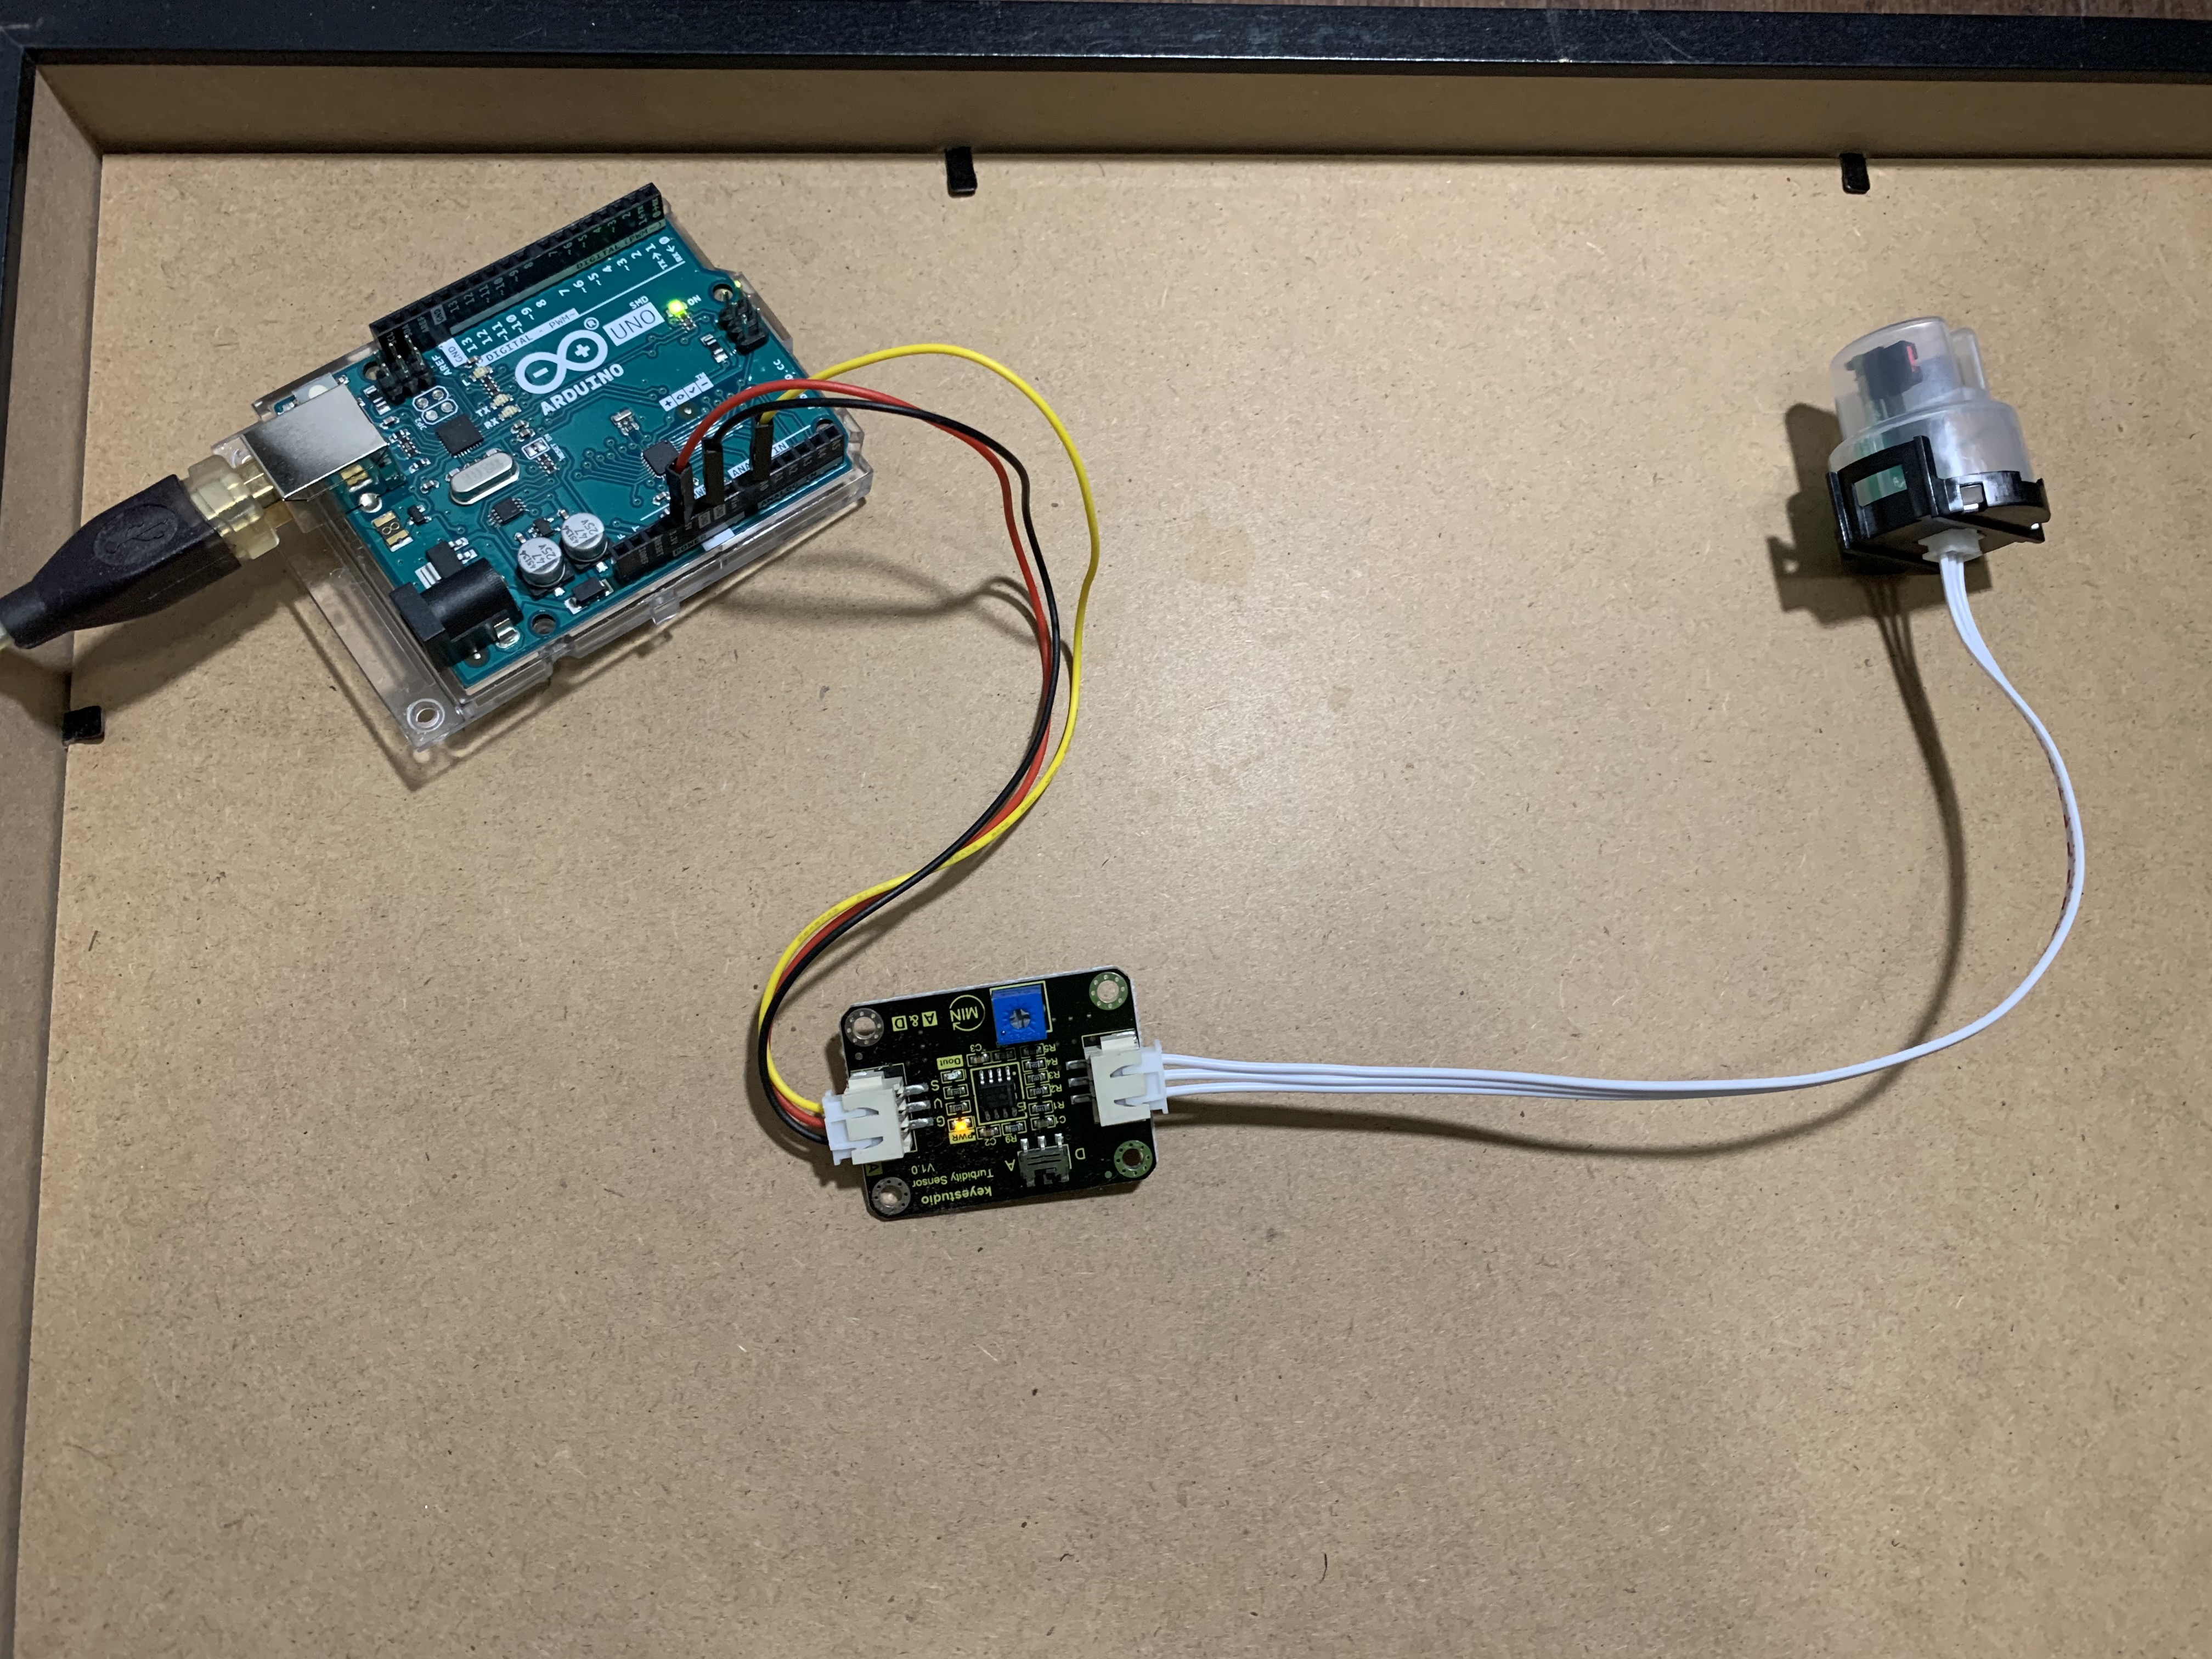
\includegraphics{C:/Users/klin/Desktop/KL/Training/Master/Courses/UoG_Bioinstrumentation/Project/Report/picture/audrui.jpg}
\caption{Figure 1: complete final tubidity meter setup}
\end{figure}

\emph{Market Analysis}

\begin{verbatim}
Drinking water and industrial water all require to pass stringent requirement prior to further using. There are many specificications that water needs to pass. One of requirement is Total Dissolved Solid (TDS) and it can measured through turbidity meter. Two types of turbidity meter are commonly used in the market including holdheld and benchtop. According to Future Market Insight, global turbidity meter will reach one billion US dollar in 2029 end. Handhold turbidity meters will reach 400 million by 2029 end. [1] This business proposal is targeting on handhold turbidity meter.  
\end{verbatim}

\emph{Current Market Competitors}

\begin{verbatim}
There are many brand companies manufacturing this device including Thermo Scientific. Lowest price is $913.5 Canadian dollars and highest one is $2224.82 canadian dollars.Since this is new product, I will make my product lowest in the  market in order to sell quickly. I will set my price as $500 Canadian dollars. After generating quick cash and will the profit to manufacture more products. 
\end{verbatim}

\begin{Shaded}
\begin{Highlighting}[]
\NormalTok{brand <-}\StringTok{ }\KeywordTok{c}\NormalTok{(}\StringTok{"Oakton"}\NormalTok{,}\StringTok{"Hach"}\NormalTok{,}\StringTok{"Extech"}\NormalTok{,}\StringTok{"Thermo Scientific"}\NormalTok{, }\StringTok{"HF Scientific"}\NormalTok{,}\StringTok{"Lovibond"}\NormalTok{)}
\NormalTok{lowest_price <-}\StringTok{ }\KeywordTok{c}\NormalTok{(}\FloatTok{1259.01}\NormalTok{, }\FloatTok{1969.92}\NormalTok{,}\FloatTok{913.5}\NormalTok{,}\FloatTok{1804.9}\NormalTok{,}\FloatTok{1565.48}\NormalTok{,}\FloatTok{1613.36}\NormalTok{)}
\NormalTok{highest_price <-}\StringTok{ }\KeywordTok{c}\NormalTok{(}\FloatTok{1617.05}\NormalTok{, }\FloatTok{1969.92}\NormalTok{,  }\FloatTok{913.5}\NormalTok{,}\FloatTok{2224.82}\NormalTok{,}\FloatTok{1565.48}\NormalTok{,}\FloatTok{1613.36}\NormalTok{)}

\NormalTok{HandheldTurbidityMeter <-}\KeywordTok{data.frame}\NormalTok{(brand,lowest_price,highest_price)}

\NormalTok{knitr}\OperatorTok{::}\KeywordTok{kable}\NormalTok{(HandheldTurbidityMeter,}\DataTypeTok{caption =} \StringTok{"Major vendors of Handheld Turbidity Meter"}\NormalTok{)}
\end{Highlighting}
\end{Shaded}

\begin{longtable}[]{@{}lrr@{}}
\caption{Major vendors of Handheld Turbidity Meter}\tabularnewline
\toprule
brand & lowest\_price & highest\_price\tabularnewline
\midrule
\endfirsthead
\toprule
brand & lowest\_price & highest\_price\tabularnewline
\midrule
\endhead
Oakton & 1259.01 & 1617.05\tabularnewline
Hach & 1969.92 & 1969.92\tabularnewline
Extech & 913.50 & 913.50\tabularnewline
Thermo Scientific & 1804.90 & 2224.82\tabularnewline
HF Scientific & 1565.48 & 1565.48\tabularnewline
Lovibond & 1613.36 & 1613.36\tabularnewline
\bottomrule
\end{longtable}

\emph{Busniess Plan}

\begin{verbatim}
In the first stage, a funding is required. Potential funding partner includes school enterpreship plan from guelph
\end{verbatim}

university. Canadian governemnt also provides funding for enterpreship.
There are many funding body in Canada govern body. {[}4{]}

\begin{Shaded}
\begin{Highlighting}[]
\NormalTok{Organization <-}\StringTok{ }\KeywordTok{c}\NormalTok{(}\StringTok{"BDC Small Business Loan"}\NormalTok{,}\StringTok{"BDC Newcomer Entrepreneur"}\NormalTok{,}\StringTok{"Canada Small Business Financicing Program"}\NormalTok{,}\StringTok{"MaRS Investment Accelerator Fund"}\NormalTok{,}\StringTok{"OCE Market Readiness Program"}\NormalTok{, }\StringTok{"OCE Voucher Programs"}\NormalTok{)}

\NormalTok{Govern_body <-}\StringTok{ }\KeywordTok{c}\NormalTok{(}\StringTok{"Federal"}\NormalTok{,}\StringTok{"Federal"}\NormalTok{,}\StringTok{"Federal"}\NormalTok{,}\StringTok{"Ontario"}\NormalTok{,}\StringTok{"Ontario"}\NormalTok{,}\StringTok{"Ontario"}\NormalTok{)}

\NormalTok{funding_body <-}\StringTok{ }\KeywordTok{data.frame}\NormalTok{(Organization,Govern_body)}

\NormalTok{knitr}\OperatorTok{::}\KeywordTok{kable}\NormalTok{(funding_body,}\DataTypeTok{caption =} \StringTok{"Potential Funding bodies for Turbidity Meter Startup"}\NormalTok{)}
\end{Highlighting}
\end{Shaded}

\begin{longtable}[]{@{}ll@{}}
\caption{Potential Funding bodies for Turbidity Meter
Startup}\tabularnewline
\toprule
Organization & Govern\_body\tabularnewline
\midrule
\endfirsthead
\toprule
Organization & Govern\_body\tabularnewline
\midrule
\endhead
BDC Small Business Loan & Federal\tabularnewline
BDC Newcomer Entrepreneur & Federal\tabularnewline
Canada Small Business Financicing Program & Federal\tabularnewline
MaRS Investment Accelerator Fund & Ontario\tabularnewline
OCE Market Readiness Program & Ontario\tabularnewline
OCE Voucher Programs & Ontario\tabularnewline
\bottomrule
\end{longtable}

\begin{verbatim}
 Second stage is manufactuing sample step, we will manufacture just a few samples by myself for demostration only. I can just use my garage to assembly turbidity meter.  

 Third stage is marketing step,I will call all of water related company to see they wants to try our new product. Below shows potential customers. In the early stage, I will send out emails to them or call them to promote this product. 
 
 
\end{verbatim}

\begin{Shaded}
\begin{Highlighting}[]
\NormalTok{Company  <-}\StringTok{ }\KeywordTok{c}\NormalTok{(}\StringTok{"Protected Elsius"}\NormalTok{,}\StringTok{"Genome Alberta"}\NormalTok{,}\StringTok{"Xenon Pharmaceuticals Inc"}\NormalTok{, }\StringTok{"Takeda Canada Inc"}\NormalTok{,}\StringTok{"BIOTECanada"}\NormalTok{,}\StringTok{"MaRS Discovery District"}\NormalTok{,}\StringTok{"University of Waterloo"}\NormalTok{,}\StringTok{"Merck Canada"}\NormalTok{,}\StringTok{"Pfizer Canada Inc"}\NormalTok{,}\StringTok{"Valeant Canada"}\NormalTok{,}\StringTok{"BioAuxilium Research"}\NormalTok{)}
\NormalTok{Location <-}\StringTok{ }\KeywordTok{c}\NormalTok{(}\StringTok{"Alberta:Calgary"}\NormalTok{,}\StringTok{"Alberta:Calgary"}\NormalTok{,}\StringTok{"British Columbia:Burnaby"}\NormalTok{,}\StringTok{"Ontarion:Oakville"}\NormalTok{,}\StringTok{"Ontario:Ottawa"}\NormalTok{,}\StringTok{"Ontario:Toronto"}\NormalTok{,}\StringTok{"Ontario :Waterloo"}\NormalTok{,}\StringTok{"Quebec:Kirkland"}\NormalTok{,}\StringTok{"Quebec:Kirkland"}\NormalTok{,}\StringTok{"Quebec:Montreal"}\NormalTok{,}\StringTok{"Quebec:St Laurent"}\NormalTok{)}
\NormalTok{Category <-}\StringTok{ }\KeywordTok{c}\NormalTok{(}\StringTok{"Industry Service & Support"}\NormalTok{,}\StringTok{"Early stage biotechnology"}\NormalTok{,}\StringTok{"Early stage biotechnology"}\NormalTok{,}\StringTok{"Commercial biotechnolgoy"}\NormalTok{,}\StringTok{"Industry Organization"}\NormalTok{,}\StringTok{"Incubator & Accelerator"}\NormalTok{,}\StringTok{"Research and Academia"}\NormalTok{,}\StringTok{"Commercial biotechnology"}\NormalTok{,}\StringTok{"Commercial biotechnology"}\NormalTok{, }\StringTok{"Industry Service & Support"}\NormalTok{,}\StringTok{"Commercial biotechnology"}\NormalTok{)}
\NormalTok{customers <-}\StringTok{ }\KeywordTok{data.frame}\NormalTok{(Company,Location,Category)}

\NormalTok{knitr}\OperatorTok{::}\KeywordTok{kable}\NormalTok{(customers)}
\end{Highlighting}
\end{Shaded}

\begin{longtable}[]{@{}lll@{}}
\toprule
Company & Location & Category\tabularnewline
\midrule
\endhead
Protected Elsius & Alberta:Calgary & Industry Service \&
Support\tabularnewline
Genome Alberta & Alberta:Calgary & Early stage
biotechnology\tabularnewline
Xenon Pharmaceuticals Inc & British Columbia:Burnaby & Early stage
biotechnology\tabularnewline
Takeda Canada Inc & Ontarion:Oakville & Commercial
biotechnolgoy\tabularnewline
BIOTECanada & Ontario:Ottawa & Industry Organization\tabularnewline
MaRS Discovery District & Ontario:Toronto & Incubator \&
Accelerator\tabularnewline
University of Waterloo & Ontario :Waterloo & Research and
Academia\tabularnewline
Merck Canada & Quebec:Kirkland & Commercial biotechnology\tabularnewline
Pfizer Canada Inc & Quebec:Kirkland & Commercial
biotechnology\tabularnewline
Valeant Canada & Quebec:Montreal & Industry Service \&
Support\tabularnewline
BioAuxilium Research & Quebec:St Laurent & Commercial
biotechnology\tabularnewline
\bottomrule
\end{longtable}

\begin{verbatim}
Forth stage is to proceed massive manufacture stage. A lab or manufacturing site will be used to manufacture these equipements. 
\end{verbatim}

\emph{Turbidity Meter Circuit Design:}

\begin{verbatim}
 Principle of turbidity meter sensor is to use optic principle to estimate transmittance rate and scattering rate. It's similar to spectrometer which detects optical density. Water serves as blank for turbidity measurement. Phototransistor which is part of turbidity meter sensor and used to collect lights that pass through haze. photoresistor is the component that connects to the phototransistor. photodiodes is used to convert light into current because emitted sun light has photon. Photon is converted into electron which generates current. That's also the princinple of converting solar energy into electricity.  If light density is higher, it wil have hight signal. After it collects the light, it will generate current. It can be collected to a resistor followed by op-amp to boost signal. The output of phototransitor is defined as base area of it and current gain of transitor. The sensing element of turbidity sensor is photodiode. First, it generates signal in the order of uA. A high-gain, low-noise transimpdedance amplifier which is operational amplifier strength signal followed by low pass filter. Analouge to digital converter to interface of microcontroller. 
 
 

 Sample has higher amount of haze or total suspended solid(TSS) will decrease light transmittance meaning the turbidity sensor reading is lower. Sample with lower amount of haze will have increase reading. The unit for turbidity meter is NTU.
 
The general flow of detecting equipment is sensing element, signal conditioning, filter, analog to digital converter and microcontroler. There are two turbididty sensors have been used in this project and comparison will be done to verify which one outperform (Figure 1-3). Analog signal output is sinusoidal and digital signal output is square signal in binary format. In otherwords latter one is discrete value. Keyestudio sensor has ability to change between these two modes. Analog signal band pass is low but digital signal band pass is high.   


  Turbidity sensor has connected it analogous controller to obtain sensor reading. This signal needs to be furhter manipulated conditioned into human readable data. In this case, Analougue controller is connected to Arduino. Arduino is connected to a laptop using a cable. Software Arduino is downloaded. The reading is voltage and needs to change to NTU. The formula to convert voltage to NTU is: 
 
\end{verbatim}

NTU = -1120.4\emph{\(\sqrt(voltage)\) + 5742.3}voltage - 4353.8

Any non-dissolved material in water can increase turbidity. when the
light pass through photodiode to phototransitor in water, amount of
light pass through depends on the total suspended solid.

Alt-Reference

{[}1{]} S. Ramesh, M. Sivaramakrishna, G. Rao. Design and development of
a quasi-digital sensor and instrument for water turbidity
measurement,Measurement Science and Technology, vol.~30, p.~115106, 2019

{[}1{]}
\url{https://www.futuremarketinsights.com/reports/turbidimeter-market}.
03/05/2020

{[}2{]} \url{https://www.coleparmer.ca/c/turbidity-meters}. 03/05/2020.

{[}3{]} \url{http://www.biotech.ca/biolist/}. 03/05/2020.

{[}4{]}
\url{https://innovation.ised-isde.canada.ca/s/group-groupe?language=en_CA\&token=a0B5W000000ArMcUAK.03/05/2020}

{[}5{]}
\url{https://www.mentorworks.ca/what-we-offer/government-funding/funding-regions/ontario/}
. 03/05/2020


\end{document}
